\input{/Users/daniel/github/config/preamble.sty}%This is available at github.com/danimalabares/config

\usepackage[style=authortitle-terse,backend=bibtex]{biblatex}
\addbibresource{bibliography.bib}

\begin{document}

\begin{minipage}{\textwidth}
	\begin{minipage}{1\textwidth}
		Geometria Simpl\'etica \hfill Daniel González Casanova Azuela
		
		{\small Profs. Henrique Bursztyn e Leonardo Macarini\hfill\href{https://github.com/danimalabares/sg}{github.com/danimalabares/sg}}
	\end{minipage}
\end{minipage}\vspace{.2cm}\hrule

\vspace{10pt}
{\huge Lista 4}

\tableofcontents

\addcontentsline{toc}{subsection}{Problem 1}
\begin{idea4}{Problema 1}\leavevmode
Let $M$ be a compact, connected, orientable $n$-dimensional manifold. Let $\Lambda_0,\Lambda_1\in\Omega^{n}(M)$ be two volume forms on $M$ such that $\int_{M}\Lambda_0=\int_{M}\Lambda_1$. Show that there is a diffeomorphism $\phi \in \operatorname{Dif}(M)$ such that $\phi^*\left( \Lambda_1 \right) =\Lambda_0$.
\end{idea4}

\begin{proof}[Solução]
Aqui sigo as definições em \cite{lee}, p. 380.  Como $M$ é orientada, em cada ponto podemos pegar um marco orientado (i.e. que em cada ponto pertence à clase de equivalencia dada pela orientação) $E_1,\ldots,E_n$ tal que as formas $\Lambda_0$ e $\Lambda_1$ são sempre positivas ou sempre negativas. Mas ainda, como $\int_{M}\Lambda_0=\int_{M}\Lambda_1>0$,
\[\Lambda_0(E_1,\ldots,E_0),\Lambda(E_1,\ldots,E_n)>0\]
para qualquer marco orientado. Daí é claro que $\Lambda_t(E_1,\ldots,E_n)>0$, de modo que $\Lambda_t$ não pode ser a forma zero em nenhum ponto de $M$, i.e. é uma forma de volumen.

	Para ver que $\left[ \Lambda_0 \right] =\left[ \Lambda_1 \right] $ lembre que $H^{n}(M)$ tem dimensão 1. Daí existe um escalar $\alpha$ tal que $\left[ \Lambda_0 \right] =\alpha \left[ \Lambda_1 \right] $. Mas, como a integral está bem definida em classes de cohomologia, $\int_{M}\left[ \Lambda_0 \right] =\int_{M}\left[ \Lambda_1 \right] \implies \alpha=1$.

Para concluir só devemos aplicar o Método de Moser. Já temos uma família de formas cohomologas, assim existe uma isotopía $ \varphi_t$ tal que $\varphi^*_{t}\Lambda_t=\Lambda_0$. Pegando $t=1$ obtemos o difeomorfismo buscado.
\end{proof}

\addcontentsline{toc}{subsection}{Problem 2}
\begin{idea8}{Problem 2}\leavevmode
	Give an example of two symplectic forms on $\mathbb{R}^{4}$ that induce the same orientation, but admit a convex combination that is degenerate. Is it possible to find an example like that, but admitting another of \textit{symplectic} forms from one to the other? What happens if we consider $\mathbb{R}^{2}$ instead of $\mathbb{R}^{4}$?
\end{idea8}

\begin{proof}[Solução]\leavevmode
	{\color{2} (See \href{https://math.stackexchange.com/questions/2864834/non-linear-path-between-symplectic-forms-in-mathbbr4}{StackExchange}.)}\hspace{1em} Lembre que no problema 1 da lista 1 vimos que uma 2-forma $\omega$ é não degenerada se é só se $\omega^n\neq 0$. No nosso caso, qualquer 2-forma em $\mathbb{R}^{4}$ pode ser expressada como
	\[\omega = \alpha \, dx \wedge dy + \beta \, dx \wedge dz + \gamma \, dx \wedge dw + \delta \, dy \wedge dz + \varepsilon \, dy \wedge dw + \phi \, dz \wedge dw \, .\]
	Daí,
	\[\omega \wedge \omega =2 F \, dx \wedge dy \wedge dz \wedge dw\]
	onde $F = \alpha \phi - \beta \varepsilon + \gamma \delta$ (vou fazer essa conta num caso análogo abaixo). Segue que $\omega$ é não degenerada se e só se $F\neq 0$.

	Nosso primeiro problema é achar $\omega_0$ e $\omega_1$ tais que as suas funções associadas como acima, $F_0$ e $F_1$, sejam não-zero, mas que exista uma combinação convexa delas $\omega_t$ cuja função $F_t$ sim seja zero. Note que se $\omega_t=(1-t)\omega_0+t\omega_1$,
\begin{align*}
	\omega_t\wedge \omega_t&=\Big( (1-t)\omega_0+t\omega_1 \Big) \wedge \Big( (1-t)\omega_0+t \omega_1 \Big) \\
	&=(1-t)^2\omega_0\wedge \omega_0 +t(1-t)\Big(\omega_0\wedge \omega_1+\omega_1\wedge \omega_0\Big)+t^2\omega_1\wedge \omega_1\\
	&=(1-t)^2\omega_0\wedge \omega_0+\Big(2t(1-t)\Big)\omega_0\wedge \omega_1+t^2\omega_1\wedge \omega_1
\end{align*}
Agora vou calcular $\omega_0\wedge \omega_1$:
\begin{align*}
	&\omega_0\wedge \omega_1\\
	&=\Big( \alpha_1 \, dx \wedge dy + \beta_1 \, dx \wedge dz + \gamma_1 \, dx \wedge dw + \delta_1 \, dy \wedge dz + \varepsilon_1 \, dy \wedge dw + \phi_1 \, dz \wedge dw \Big)\\
	&\wedge \Big( \alpha_2 \, dx \wedge dy + \beta_2 \, dx \wedge dz + \gamma_2 \, dx \wedge dw + \delta_2 \, dy \wedge dz + \varepsilon_2 \, dy \wedge dw + \phi_2 \, dz \wedge dw \Big) \\
	&= 2\alpha_1 \phi_2dx\wedge dy\wedge dz\wedge dw+\;2\beta_1\varepsilon_2 dx\wedge dz\wedge dy\wedge dw+\; 2\gamma_1\delta_2dx\wedge dw \wedge dy\wedge dz
\end{align*}
de forma que
\[\omega_0\wedge \omega_1=2\Big(\alpha_1\phi_2-\beta_1 \varepsilon_2+\gamma_1 \delta_2\Big)dx\wedge dy\wedge dz\wedge d\]
Definamos $F_{01}:=\alpha_1\phi_2-\beta_1 \varepsilon_2+\gamma_1 \delta_2$.

Agora pegue $\alpha_1=\alpha_2=\phi_1=\phi_2=\beta_1=1$, $\varepsilon_2=2$ e o resto zero. Obtemosque $F_0=F_1=1$, e que $F_{01}=-1$. Então
\begin{align*}
\omega_t\wedge \omega_t&=2\left( (1-t)^2-2t(1-t)+t^2 \right)  dx\wedge dy\wedge dz\wedge dw\\
&=2\Big( 1-2t+t^2-2t+2t^2+t^2 \Big)dx\wedge dy\wedge dz\wedge dw\\
&=2\Big( 1-4t+4t^2 \Big)dx\wedge dy\wedge dz\wedge dw\\
&=2(1-2t)^2dx\wedge dy\wedge dz\wedge dw
\end{align*}
Por fim, $\omega_t$ é degenerada quando $t=1/2$.

Para mostrar que existe uma trajetória de formas simpléticas conectando $\omega_0$ e $\omega_1$ note que o espaço de 2-formas pode ser identificado com $\mathbb{R}^{6}$ com coordenadas $(\alpha,\beta,\gamma,\delta,\varepsilon,\phi)$. Pelas observações anteriores, vemos que o conjunto de formas degeneradas é a variedade (algébrica) $[F=0]$. Duas formas determinan a mesma  orientação quando estão no mesmo conjunto $[F>0]$ ou  $[F<0]$. Por exemplo, as formas $\omega_0$ e $\omega_1$ estão em $[F>0]$.

Mostrar que existe um caminho que conecta essas formas (o quaisquer duas que induzam a mesma orientação) é tanto como mostrar que $[F>0]$ (e $[F<0]$) é un conjunto conexo. Aseguir mostrarei que de fato a variedade $[F=0]$ separa  $\mathbb{R}^{6}$ em duas componentes conexas $[F>0]$ e  $[F<0]$.

Primeiro note que o gradiente de  $F$ é $\nabla F=(\phi,-\varepsilon,\delta, \gamma,-\beta,\alpha)$. Ele é não-zero em $\mathbb{R}^{6}\setminus 0$, de modo que, $[F=0]\setminus 0$ é uma variedade suave. Como $0\in [F=0]$, podemos fixar nossa atenção em $\mathbb{R}^{6}\setminus 0$, que é um retrato por deformação de $S^5\subset \mathbb{R}^{6}$ e mostrar que $F|_{S^5}$ induiz duas componentes conexas.

Como $S^5$ é compacto, $F|_{S^5}$ tem pelo menos um máximo local em $[F>0]$ e um mínimo local em $[F<0]$. Note que dado um ponto no conjunto $[F>0]$, existe um caminho, determinado pelo gradiente, que conduiz até um ponto máximo local dentro de $[F>0]$. Dados dois pontos em  $[F>0]$, podemos achar um caminho entre eles dentro de  $[F>0]$ se conseguimos mostrar que qualquer par de maximos locais  está conectado por um caminho dentro de $[F>0]$.  O mesmo acontece para pontos em $[F<0]$.  Então a prova está concluida se mostramos que os pontos críticos (máximos ou mínimos) de $F$ estão na mesma componente conexa (i.e. $[F>0]$ ou  $[F<0]$, respectivamente).

Como $\nabla F$ é um vetor que aponta na direção de maior pendente, um ponto $p \in S^5$ é critico se e só se $\nabla F_p$ é paralelo $p$. Podemos ver $\nabla F$ como uma transformação linear $\mathbb{R}^{6}\longrightarrow \mathbb{R}^{6}$, $p \mapsto \nabla_p F$. De fato, ela é dada pela matriz $H$ que tem $(1,-1,1,-1,1)$ na antidiagonal e zero no resto. Então vemos que os pontos críticos são exatamente os vetores próprios dessa matriz.

Fazendo as \href{https://www.wolframalpha.com/input?i=%7B%7B0%2C0%2C0%2C0%2C0%2C1%7D%2C%7B0%2C0%2C0%2C0%2C%E2%88%921%2C0%7D%2C%7B0%2C0%2C0%2C1%2C0%2C0%7D%2C%7B0%2C0%2C1%2C0%2C0%2C0%7D%2C%7B0%2C%E2%88%921%2C0%2C0%2C0%2C0%7D%2C%7B1%2C0%2C0%2C0%2C0%2C0%7D%7D+&lang=es}{contas} de álgebra linear, pode comprovar que os valores próprios de $H$ são $\pm 1$, cada um com multiplicade 3. Assim, temos dois espaços próprios de dimensão 3. Quando intersectamos esses espaços com $S^5$, obtemos duas esferas de dimensão 2. Essas esferas são disjuntas e conexas, e representas os conjuntos de pontos críticos de $F$.

{\color{1}\bfseries Uma solução mais terrenal.}\hspace{1em}Contudo, uma prova mais directa consiste em observar o seguinte: os valores de $\beta_1$ e $\varepsilon_2$ não alteram o fato de que as formas $\omega_0$ e $\omega_1$ sejam formas não degeneradas (e que induzem a mesma orientação), enquanto que $\omega_t\wedge \omega_t$ sí pode mudar. Vamos mostrar que as formas $\omega_0$ e $\omega_1$ definidas acima podem ser conectadas por um caminho de formas simpléticas trocando $\beta_1$ e $\varepsilon_0$ por funções de $t$.

Primeiro fixe os mesmos valores $\alpha_1,\alpha_2,\ldots$ como no caso anterior, mas deixe $\beta_1$ e $\varepsilon_2$ sem definir. Obtemos que:
\begin{align*}
\omega_t\wedge \omega_t&=2\left( (1-t)^2+2t(1-t)\beta_1\varepsilon_2+t^2 \right)  dx\wedge dy\wedge dz\wedge dw\\
&=2\Big( 1-2t+t^2+2t\beta_1\varepsilon_2-2t^2\beta_1\varepsilon_2+t^2 \Big)dx\wedge dy\wedge dz\wedge dw\\
&=2\Big((2-2\beta_1\varepsilon_2)t^2-2t(\beta_1\varepsilon_2-1)t+1\Big)dx\wedge dy\wedge dz\wedge dw
\end{align*}
Agora defina
\begin{align*}
	\beta_1=-2(t-1/2),\qquad \qquad \varepsilon_0=4(t-1/2) 
\end{align*}
e considere a família de formas  $\omega'_t=(1-t)\omega_0(t) \omega_1(t)$. Note que $\omega_0'=\omega_0$ e $\omega_1'=\omega_1$. Daí,
\begin{align*}
\omega_t\wedge \omega_t&=2\Bigg(\big((2-2\big(\underbrace{-2(t-1/2)}_{\beta_1}\big)\underbrace{4(t-1/2)}_{\varepsilon_2}\big)t^2\\
&\; \;-2t\Big(\big(\underbrace{-2(t-1/2)}_{\beta_1}\big)\underbrace{4(t-1/2)}_{\varepsilon_2}-1\Big)t+1\Bigg)dx\wedge dy\wedge dz\wedge dw
\end{align*}
Para calcular isso calculei que
\[\beta_1\varepsilon_2=-8t^2-4t+1\]
daí cheguei a que
\[\omega_t\wedge \omega_t=2\big(32t^4-32t^3+6t^2+1\big)dx\wedge dy\wedge dz\wedge dw\]
de modo que $F_t$ nunca se anula.
\begin{figure}[H]
	\centering
	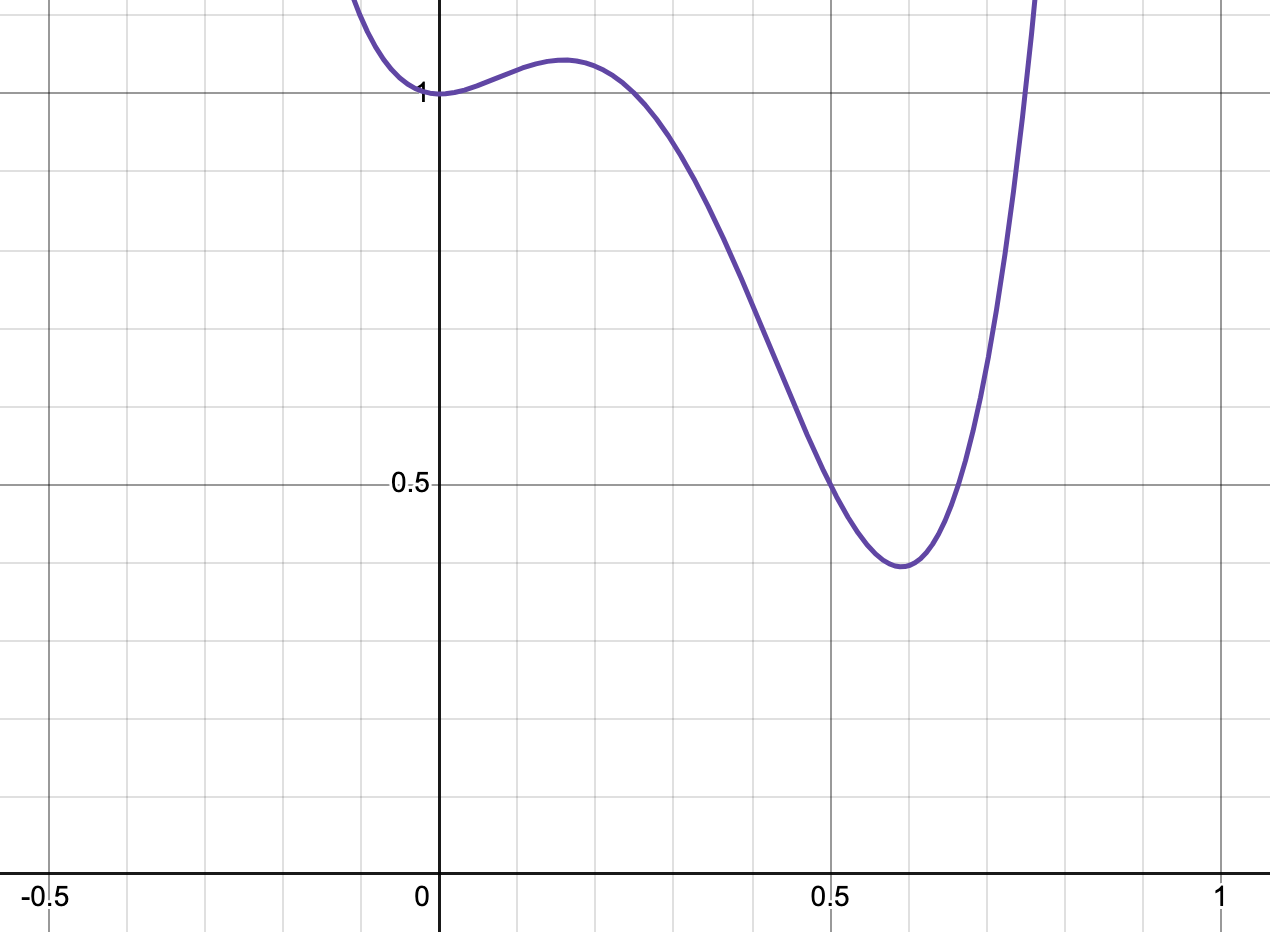
\includegraphics[width=0.4\textwidth]{fig1}
	\caption*{$F_t$}
\end{figure}

Em fim, no caso de $\mathbb{R}^{2}$, suponha que $\omega_0$ e $\omega_1$ são duas formas não degeneradas. Sabemos que em qualquer ponto de $\mathbb{R}^{2}$ elas são um múltiplo da outra. Portanto, uma combinação convexa delas não pode ser degenerada porque é da forma
\[\omega_t=(1-t)\omega_0+t\lambda\omega_0=(1-t+\lambda t)\omega_0.\]
\end{proof}

\addcontentsline{toc}{subsection}{Problem 3}
\begin{idea5}{Problem 3}\leavevmode
Let $(V,\Omega)$ be a symplectic vector space (or vector bundle) and let $W\subseteq V$ be a coisotropic subspace (or bundle).
\begin{enumerate}[label=\alph*.]
	\item Let $E$ be a complement of $W^\Omega$ in $W$, i.e., $W=W^\Omega\oplus E$. Show that the restriction of $\Omega$ to $E$ is nondegenerate.
	\item Let $J$ be a $\Omega$-compatible complex structure, with $g$ the associated inner product. Show that $\Omega$ induces an identification of $J(W^\Omega)=W^\perp$ with $(W^\Omega)^*$. Taking $E$ as the orthogonal complement (with respect to $g$) to $W^\Omega$ in $W$ (this means that $W=W^\Omega\oplus E$), show that the identification
		\[V\cong E\oplus (W^\Omega\oplus (W^\Omega)^*),\]
		is an isomorphism of symplectiv vector spaces (bundles)---on the right-hand-side, $E$ is equipped with its induced symplectic form (see a. above) and $W^\Omega\oplus (W^\Omega)^*$  with its canonical symplectic form.
\end{enumerate}
\end{idea5}

\begin{proof}[Solução]\leavevmode 
\begin{enumerate}[label=\alph*.]
	\item 	Basta ver que $\ker \Omega|_{E}=0$. Se $e\in\ker \Omega|_{E}$, então eu gostaria de ver que $e\in W^\Omega$ para concluir que $e=0$. Seja $w\in W$. Então $\Omega(e,w)=\Omega(e,w_1+w_2)$ com $w_1\in W^\Omega$ e $w_2\in E$. Daí $\Omega(e,w)=0$ já que tanto $\Omega(e,w_1)=0$ porque $e\in E\subset W$ quanto $\Omega(e,w_2)=0$ porque $w_2\in E$.

	\item Considere o mapa
		\begin{align*}
			J(W^\Omega) &\longrightarrow (W^\Omega)^* \\
			Jw &\longmapsto i_w\Omega= \Omega(w,\cdot )
		\end{align*}
		Note que $J(W^\Omega)$ e $W^\Omega$ são espaços vetorias de dimensões iguais, e que esse mapa tem kernel trivial pela não degeneração de $\Omega$. Isso explica que é um isomorfismo.

	Para construir o isomorfismo requerido note que por definição $W\cong E\oplus W^\Omega$. E como mostramos que $W^\perp\cong (W^\Omega)^*$, sabemos que $V\cong W\oplus (W^\Omega)^*$. Daí o isomorfismo algébrico está comprovado por causa de que a soma direita é associativa. Issto é, temos um isomorfismo de espaços vetoriais
	\begin{align*}
		\Phi: V &\longrightarrow E\oplus W^\Omega\oplus (W^\Omega)^* \\
		v &\longmapsto (v_1,v_2,v_3)
	\end{align*}
	onde $g(v_1,v_2)=0$ e $g(v_1+v_2,v_3)=0$.

	Agora vamos comprovar que esse mapa é um simplectomorfismo, 
	
\end{enumerate}
\end{proof}

\addcontentsline{toc}{subsection}{Problem 4}
\paragraph{Problem 4}Prove the following generalizaion of Weinstein's lagrangian neighbourhood theorem to coisotropic submanifolds (due to Gotay, 1982): Let $(M_0,\omega_0)$ be and $(M_1,\omega_1)$ be symplectic manifolds, and $\iota_0:Q\longrightarrow M_0$, $\iota_1:Q\longrightarrow M_1$ be coisotropic embeddings. If $\iota^*_0\omega_0=\iota_1^*\omega_1$ then there exist open  neighbourhoods $\mathcal{U}_0$ and $\mathcal{U}_1$ of $Q$, in $M_0$ and $M_1$, and a diffeomorphism $\varphi:\mathcal{U}_0\longrightarrow \mathcal{U}_1$ such that $\varphi(p)=p$ for all $p\in Q$ and $\varphi^*\omega_1=\omega_0$.

\begin{proof}[Solução]\leavevmode
	Estamos aqui:
	\[\begin{tikzcd}
		(M_0,\omega_0)&&(M_1,\omega_1)\\
	&Q\arrow[ul,"\iota_0",hook]\arrow[ur,"\iota_1",hook,swap]
	\end{tikzcd}\]
Em aula demostramos que:
\begin{thm}[Teorema de Darboux generalizado Vers\~ao 2.0]\leavevmode
	Suponha que, além do diagrama anterior, temos um isomorfismo de fibrados simpl\'ecticos
	\[\begin{tikzcd}
	TM_0|_{Q}\arrow[rr,"\phi"]\arrow[dr,swap]&&TM_1|_{Q}\arrow[dl]\\
	&Q
	\end{tikzcd}\]
	tal que $\phi|_{TQ}:TQ\to TQ$ é $\operatorname{id}_{TQ}$.

	Ent\~ao $\phi$ estende a derivada de um simplectomorfismo
	\[\begin{tikzcd}
	U_0\subset M_0\arrow[rr,"\varphi"]&&U_1\subset M_1\\
	&Q\arrow[ul]\arrow[ur,swap]
	\end{tikzcd}\]
	i.e.,
	\[d\varphi|_{Q}=\phi:TM_0|_{Q}\to TM_1|_{Q}\]
	Em palavras: a derivada do simplectomofismo (entre as vizinhanças de $M_1$ e $M_2$) que obtemos é estendida pelo isomorfismo simpl\'etico dos fibrados tangentes que nos foi dado.
\end{thm}
Portanto, para nosso exercício só precisamos achar um simplectomorfismo $\phi$ de fibrados tangentes que restringe a identidade no $TQ$.

Também é bom lembrar que na prova do teorema das vizinhanças lagrangianas construiimos esse simplectomorfismo de fibrados do seguinte jeito:
	\[\begin{tikzcd}
	&T\mathcal{L}\oplus (T\mathcal{L})^*\arrow[dr,"\cong "]\\
	TM|_{\mathcal{L}}\arrow[rr,"\phi"]\arrow[ur,"\cong "]&&T(T^*\mathcal{L})|_{\mathcal{L}}
	\end{tikzcd}\]
	Issto é, mostrando que, no caso lagragiano, existe um isomorfismo de fibrados tangentes entre o fibrado tangente da variedade ambiente restrito à subvariedade lagrangiana e a soma direita $T\mathcal{L}\oplus (T\mathcal{L})^*$. Aplicando isso usando como variedade ambiente tanto $M$ quanto $T^*M$ construimos o diagrama anterior.

	A estrutura complexa foi usada para obter a descomposição $T\mathcal{L}\oplus (T\mathcal{L})^*$: o que fizemos foi construir o complemento ortogonal usando a métrica compatível e daí mostramos que esse complemento é de fato isomorfo a $(T\mathcal{L})^*$.

	No caso coisotrópico temos, pelo exercício anterior, dois isomorfismos de fibrados
\begin{align*}TM_1\cong E_1\oplus \Big(TQ^\omega\oplus (TQ^\omega)^*\Big),\qquad \qquad 
TM_2&\cong E_2\oplus \Big(TQ^\omega\oplus (TQ^\omega)^*\Big)
\end{align*}
então é claro que se $E_1\cong E_2$ terminhamos. Mas $E_i$ é só o complemento ortogonal de $TQ^\omega$ respeito à métrica compatível $g_i$ em $TQ$, enquanto $g_1$ e $g_2$ coincidem em $TQ$ já que $\omega_1|_{Q}=\omega_2|_{Q}$ por hipótese (o pullback das incluções coincide). Note que também é imediato que a restrição desse isomorfismo a $TQ$  é a identidade.
\end{proof}

\end{document}
